\renewcommand{\theequation}{\theenumi}
\begin{enumerate}[label=\thesection.\arabic*.,ref=\thesection.\theenumi]
\numberwithin{equation}{enumi}
\begin{figure}[!ht]
\centering
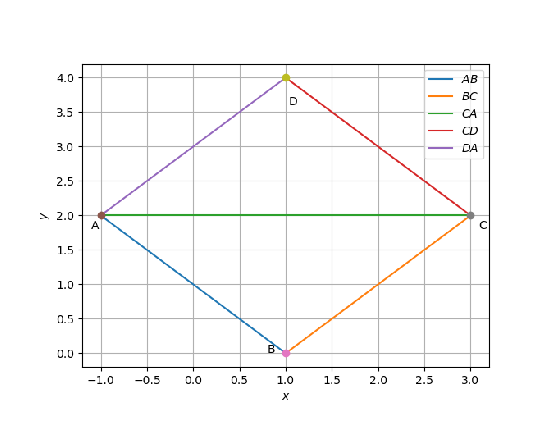
\includegraphics[width= \columnwidth]{./figs/quad/quad.eps}
\caption{Square ABCD}
\end{figure}
\item From inspection we see that the opposite vertices forms a diagonal which is parallel to x-axis. Then the diagonal formed by other two vertices is parallel to y-axis(i.e. their x coordinates are equal). Let $\vec{A}= \myvec{-1\\2}$  and $\vec{C}=\myvec{3\\2}$. In a square each interior angle is 90\degree and all sides are equal. Diagonals bisect each other at 90\degree.
Let $\vec{B}$ and $\vec{D}$ be other two vertices. If $\vec{x}$ is a vector then the given equations,
\begin{align}
\brak{\vec{x}-\vec{A}}^T\brak{\vec{x}-\vec{C}} &= 0 \\
\norm{\vec{x}-\vec{A}} &= \norm{\vec{x}-\vec{C}} 
\end{align}
are satisfied by $\vec{B}$ and $\vec{D}$. Substituting it in the given equations and solving, we get
\begin{align}
\vec{B}&= \myvec{1\\0} \\
\vec{D}&= \myvec{1\\4}
\end{align} 
\item The python code for the figure can be downloaded from
\begin{lstlisting}
codes/quad/quad.py
\end{lstlisting}
\end{enumerate}  